
%%%%%%%%%%%%%%%%%%%%%%%%%%%%%%%%%%%%%%%%%%%%%%%%%%%%%%%%
%
% Copyright (c) 2003-2009 by University of Queensland
% Earth Systems Science Computational Center (ESSCC)
% http://www.uq.edu.au/esscc
%
% Primary Business: Queensland, Australia
% Licensed under the Open Software License version 3.0
% http://www.opensource.org/licenses/osl-3.0.php
%
%%%%%%%%%%%%%%%%%%%%%%%%%%%%%%%%%%%%%%%%%%%%%%%%%%%%%%%%

\documentclass{manual}
%%% Table of contents to list down to subsections and no further
\setcounter{tocdepth}{3}
%%% Number down to subsubsections only
\setcounter{secnumdepth}{3}
% grab the handy definitions and \usepackage statements etc

%%%%%%%%%%%%%%%%%%%%%%%%%%%%%%%%%%%%%%%%%%%%%%%%%%%%%%%%%%%%%%%%%%%%%%%%%%%%%%
% Copyright (c) 2003-2018 by The University of Queensland
% http://www.uq.edu.au
%
% Primary Business: Queensland, Australia
% Licensed under the Apache License, version 2.0
% http://www.apache.org/licenses/LICENSE-2.0
%
% Development until 2012 by Earth Systems Science Computational Center (ESSCC)
% Development 2012-2013 by School of Earth Sciences
% Development from 2014 by Centre for Geoscience Computing (GeoComp)
%
%%%%%%%%%%%%%%%%%%%%%%%%%%%%%%%%%%%%%%%%%%%%%%%%%%%%%%%%%%%%%%%%%%%%%%%%%%%%%%

\usepackage{subfigure}
\usepackage{epsfig}

\usepackage{graphicx,color}
% \usepackage[pdftex]{graphicx,color}
\usepackage{makeidx}  % handle the index properly
\usepackage{xspace}   % handle spaces after commands more nicely
% use the ams math stuff, as it makes the maths easier to code, and
% nicer output than the standard LaTeX stuff
\usepackage{amsmath,amsfonts,amssymb} % this is handy for mathematicians and physici % see http://www.ams.org/tex/amslatex.html
\usepackage{alltt}   % handy verbatim stuff
\usepackage{textcomp}
\usepackage{setspace}
%\usepackage{movie15}
% Special Formatting Packages
% Colour Package
\usepackage[usenames,dvipsnames]{xcolor}
% Assignm Colour Names and import hyperlinks.
\usepackage{float}
%\usepackage[unicode,colorlinks=true,linkcolor=NavyBlue,citecolor=OliveGreen,urlcolor=Plum]{hyperref}

% Fancy Verb


\usepackage[numbers]{natbib}
\usepackage{chapterbib}
\renewcommand{\bibname}{References}

%\doublespacing

%\include{pythonlisting}

%%%%%%%%%%%%%%%%%%%%%%%%%%%%%%%%%%%%%%%%%%%%%%%%%%%%%%%%%%%%%%%%%%%%%%%%%%%%%%
% Copyright (c) 2003-2026 by the esys.escript Group
% https://github.com/LutzGross/esys-escript.github.io
%
% Primary Business: Queensland, Australia
% Licensed under the Apache License, version 2.0
% http://www.apache.org/licenses/LICENSE-2.0
%
% See CREDITS file for contributors and development history
%
%%%%%%%%%%%%%%%%%%%%%%%%%%%%%%%%%%%%%%%%%%%%%%%%%%%%%%%%%%%%%%%%%%%%%%%%%%%%%%

\usepackage{listing}
% defines the colour for the background of code examples
\definecolor{LightGrey}{gray}{0.9}

%Some colour definitions added to keep pdflatex happy
%I make no claim that these values are particularly good
\definecolor{Purple}{rgb}{0.7, 0, 0.6}
\definecolor{Tan}{rgb}{0.5,0.5,0.5}
\definecolor{BrickRed}{rgb}{0.7, 0.2, 0.2}
\definecolor{Black}{rgb}{0, 0, 0}

% All the \color{x} used to be \color[named]{x}
%end color defs

\lstdefinestyle{myC++}{%
language=C++,
showstringspaces=false,
basicstyle=\small\ttfamily,
commentstyle=\color{BrickRed}\ttfamily,
keywordstyle=\color{Purple}\ttfamily,
%identifierstyle=\color{Blue}\ttfamily,
%functionstyle=\color{Blue}\ttfamily,
%typestyle=\color{ForestGreen}\ttfamily,
stringstyle=\color{Tan}\ttfamily,%
morekeywords={,complex,}%
frame=none,%
backgroundcolor=\color{LightGrey}%
}

\lstdefinestyle{myMatlab}{%
language=Matlab,
showstringspaces=false,
basicstyle=\small\ttfamily,
commentstyle=\color{BrickRed}\ttfamily,
keywordstyle=\color{Purple}\ttfamily,
%identifierstyle=\color{Blue}\ttfamily,
%functionstyle=\color{Blue}\ttfamily,
%typestyle=\color{ForestGreen}\ttfamily,
stringstyle=\color{Tan}\ttfamily,%
frame=none,%
backgroundcolor=\color{LightGrey}%
}

\lstdefinestyle{myScilab}{%
language=Scilab,
showstringspaces=false,
basicstyle=\small\ttfamily,
commentstyle=\color{BrickRed}\ttfamily,
keywordstyle=\color{Purple}\ttfamily,
%identifierstyle=\color{Blue}\ttfamily,
%functionstyle=\color{Blue}\ttfamily,
%typestyle=\color{ForestGreen}\ttfamily,
stringstyle=\color{Tan}\ttfamily,%
frame=none,%
backgroundcolor=\color{LightGrey}%
}

\lstdefinestyle{myShell}{%
language=ksh,
showstringspaces=false,
basicstyle=\small\ttfamily,
commentstyle=\color{Black}\ttfamily,
keywordstyle=\color{Black}\ttfamily,
%identifierstyle=\color{Blue}\ttfamily,
%functionstyle=\color{Blue}\ttfamily,
%typestyle=\color{ForestGreen}\ttfamily,
stringstyle=\color{Black}\ttfamily,%
frame=none,%
backgroundcolor=\color{LightGrey}%
}

\lstdefinestyle{myFootnotesizeShell}{%
language=ksh,
showstringspaces=false,
basicstyle=\footnotesize\ttfamily,
commentstyle=\color{Black}\ttfamily,
keywordstyle=\color{Black}\ttfamily,
%identifierstyle=\color{Blue}\ttfamily,
%functionstyle=\color{Blue}\ttfamily,
%typestyle=\color{ForestGreen}\ttfamily,
stringstyle=\color{Black}\ttfamily,%
frame=none,%
backgroundcolor=\color{LightGrey}%
}

\lstdefinestyle{myPython}{%
language=python,
showstringspaces=false,
basicstyle=\small\ttfamily,
commentstyle=\color{BrickRed}\ttfamily,
keywordstyle=\color{Purple}\ttfamily,
%identifierstyle=\color{Blue}\ttfamily,
%functionstyle=\color{Blue}\ttfamily,
%typestyle=\color{ForestGreen}\ttfamily,
stringstyle=\color{Tan}\ttfamily,%
frame=none,%
%backgroundcolor=\color{LightGrey}%
}

\lstdefinestyle{myhtml}{%
language=xml,
showstringspaces=false,
basicstyle=\small\ttfamily,
commentstyle=\color{BrickRed}\ttfamily,
keywordstyle=\color{Purple}\ttfamily,
%identifierstyle=\color{Blue}\ttfamily,
%functionstyle=\color{Blue}\ttfamily,
%typestyle=\color{ForestGreen}\ttfamily,
stringstyle=\color{Tan}\ttfamily,
morekeywords={,simulation,prop_dim,error_check,stochastic,%
  globals,field,dimensions,lattice,domains,samples,vector,%
  components,fourier_space,sequence,integrate,algorithm,%
  interval,k_operators,constant,operator_names,vectors,%
  output,filename,group,sampling,moments,benchmark,use_double,%
  use_wisdom,use_prefs,binary_output,cycles,filter,post_propagation,%
  default_value,argv,arg,iterations,cross_propagation,%
  use_mpi,paths,seed,noises,author,description,name,type,%
}
frame=none,%
%framerule=2pt,%
backgroundcolor=\color{LightGrey}%
}


% this implements producing nice code blocks
% it also saves time, typing and
% *should* reduce errors in the text by removing doubling up of code
\lstnewenvironment{xmdsCode}[1][]{\lstset{style=myhtml}\lstset{#1}}{}

% this implements nicely formatted shell code
\lstnewenvironment{shellCode}[1][]{\lstset{style=myShell}\lstset{#1}}{}

% this implements nicely formatted footnotesize shell code
\lstnewenvironment{smallShellCode}[1][]{\lstset{style=myFootnotesizeShell}\lstset{#1}}{}

% this implements nicely formatted Perl code
\lstnewenvironment{perlCode}[1][]{\lstset{style=myPerl}\lstset{#1}}{}

% this implements nicely formatted Python code
\lstnewenvironment{python}[1][]{\lstset{style=myPython}\lstset{#1}}{}

% this implements nicely formatted C++ code
\lstnewenvironment{CCode}{\lstset{style=myC++}}{}

% this implements nicely formatted matlab code
\lstnewenvironment{matlabCode}{\lstset{style=myMatlab}}{}

% this implements nicely formatted scilab code
\lstnewenvironment{scilabCode}{\lstset{style=myScilab}}{}



%Ensures that latex doesn't have an error if we don't specify the version
\providecommand{\RepVersion}{Unknown\xspace}

%Tony's Commands
\newcommand{\editor}[1] {\textit{EDITORIAL: {#1}}}
\newcommand{\fileex}[1]{\module{examples\textbackslash {#1}}\xspace}
\newcommand{\TODO}[1]{\textbf{TODO}:\xspace\textit{#1} } 
\newcommand{\TBA}[1]{\textbf{TO BE ADDED: \begin{enumerate} {#1} \end{enumerate}}}
%\newcommand{\eqref}[1] {(\ref{#1})}

% text names
\newcommand{\esys}{\textit{esys}\xspace}
\newcommand{\pyt}{\textit{python}\xspace}
\newcommand{\esc}{\textit{escript}\xspace}
\newcommand{\FINLEY}{\textit{finley}\xspace}
\newcommand{\ripley}{\textit{ripley}\xspace}
\newcommand{\speckley}{\textit{speckley}\xspace}
\newcommand{\exf}{\textit{doc/examples/cookbook/}\xspace}
\newcommand{\mayavi}{\textit{Mayavi2}\xspace}

%referencing
\newcommand{\reffig}[1]{Figure~(\ref{#1})}
\newcommand{\refeq}[1]{equation~(\ref{#1})}
\newcommand{\refEq}[1]{Equation~(\ref{#1})}
\newcommand{\refCh}[1]{Chapter~\ref{#1}}
\newcommand{\refSec}[1]{Section~\ref{#1}}


%modules
\newcommand{\modesys}{\module{esys}\xspace}
\newcommand{\modescript}{\module{esys.escript}\xspace}
\newcommand{\modLPDE}{\module{esys.escript.LinearPDEs}\xspace}
\newcommand{\modfinley}{\module{esys.finley}\xspace}
\newcommand{\modpycad}{\module{esys.pycad}\xspace}
\newcommand{\modvtk}{\module{vtk}\xspace}
\newcommand{\modnumpy}{\module{numpy}\xspace}
\newcommand{\modmpl}{\module{matplotlib}\xspace}
\newcommand{\pycad}{\module{esys.pycad}\xspace}
\newcommand{\gmsh}{\module{esys.pycad.gmsh}\xspace}
\newcommand{\pylab}{\module{pylab}\xspace}
\newcommand{\mpl}{\module{matplotlib}\xspace}
\newcommand{\numpy}{\module{numpy}\xspace}
\newcommand{\weipa}{\module{esys.weipa}\xspace}

%list scripts
\newcommand{\sslist}[1]{\textbf{The scripts referenced in this section are; #1} \newline \newline}

% title, author, etc stuff
\title{The Escript COOKBOOK}

\ifpdf
\pdfinfo {
/Author (Antony Hallam and Lutz Gross)
/Title (escript COOKBOOK)
/Keywords (escript, PDEs)
}
\fi

\author{Antony Hallam, Lutz Gross}
\authoraddress{
Earth Systems Science Computational Centre (ESSCC) \\
School of Earth Sciences \\
The University of Queensland \\
Brisbane, Australia \\
Email: \email{esys@esscc.uq.edu.au}
}                                                                                         
\date{\today}      
\release{Alpha}
\setshortversion{}

\makeindex

\begin{document}

\maketitle


%%%%%%%%%%%%%%%%%%%%%%%%%%%%%%%%%%%%%%%%%%%%%%%%%%%%%%%%%%%%%%%%%%%%%%%%%%%%%%
% Copyright (c) 2003-2026 by the esys.escript Group
% https://github.com/LutzGross/esys-escript.github.io
%
% Primary Business: Queensland, Australia
% Licensed under the Apache License, version 2.0
% http://www.apache.org/licenses/LICENSE-2.0
%
% See CREDITS file for contributors and development history
%
%%%%%%%%%%%%%%%%%%%%%%%%%%%%%%%%%%%%%%%%%%%%%%%%%%%%%%%%%%%%%%%%%%%%%%%%%%%%%%

\begin{center}
Copyright (c) 2003-2026 esys.escript Group \\
\url{https://github.com/LutzGross/esys-escript.github.io}\\
Primary Business: Queensland, Australia\\
Licensed under the Apache License, version 2.0\\
\url{http://www.apache.org/licenses/LICENSE-2.0}\\
This work was supported by the AuScope National Collaborative Research
Infrastructure Strategy, the Queensland State Government and The University
of Queensland.
\end{center}



\begin{abstract}
\esc is a python-based environment that has been developed to solve complex mathematical models. These include coupled, non-linear and time-dependent partial differential equations. The intention of this cookbook, is to give new \esc users a comprehensive introduction to \esc and provide a fundamental \esc knowledge base and example set that can be used as templates for future problems. While most of the examples in this cookbook are focused on the disciplines of geophysics and geology they all provide a solid introduction to \esc and it's capabilities.  
\end{abstract}
\tableofcontents

\newpage



%%%%%%%%%%%%%%%%%%%%%%%%%%%%%%%%%%%%%%%%%%%%%%%%%%%%%%%%
%
% Copyright (c) 2003-2008 by University of Queensland
% Earth Systems Science Computational Center (ESSCC)
% http://www.uq.edu.au/esscc
%
% Primary Business: Queensland, Australia
% Licensed under the Open Software License version 3.0
% http://www.opensource.org/licenses/osl-3.0.php
%
%%%%%%%%%%%%%%%%%%%%%%%%%%%%%%%%%%%%%%%%%%%%%%%%%%%%%%%%

This document describes how to install \esfinley on your computer.
To learn how to use \esfinley please see the User guide or, for
more detailed information, the API documentation.


\chapter{Getting Started with Heat Diffusion}
\label{CHAP HEAT DIFF}

%%%%%%%%%%%%%%%%%%%%%%%%%%%%%%%%%%%%%%%%%%%%%%%%%%%%%%%%
%
% Copyright (c) 2003-2009 by University of Queensland
% Earth Systems Science Computational Center (ESSCC)
% http://www.uq.edu.au/esscc
%
% Primary Business: Queensland, Australia
% Licensed under the Open Software License version 3.0
% http://www.opensource.org/licenses/osl-3.0.php
%
%%%%%%%%%%%%%%%%%%%%%%%%%%%%%%%%%%%%%%%%%%%%%%%%%%%%%%%%

\section{One Dimensional Heat Diffusion in an Iron Rod}
%\label{Sec:1DHDv0}
We will start by examining a simple one dimensional heat diffusion example. This problem will provide a good launch pad to build our knowledge of \ESCRIPT and how to solve simple partial differential equations (PDEs)\footnote{Wikipedia provides an excellent and comprehensive introduction to \textit{Partial Differential Equations} \url{http://en.wikipedia.org/wiki/Partial_differential_equation}, however their relevance to \ESCRIPT and implementation should become a clearer as we develop our understanding further into the cookbook.}

\begin{figure}[h!]
\centerline{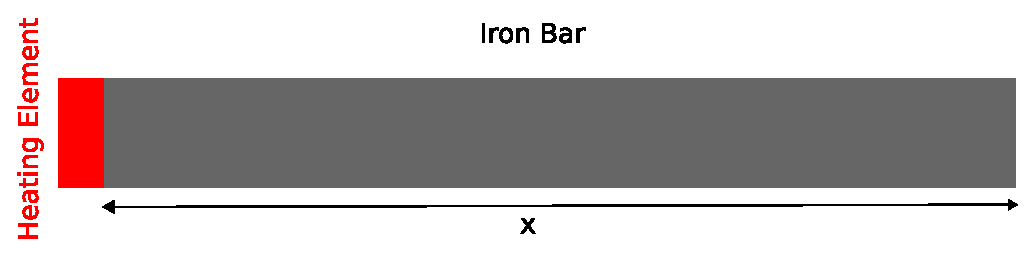
\includegraphics[width=4.in]{figures/onedheatdiff}}
\caption{One dimensional model of an Iron bar.}
\label{fig:onedhdmodel}
\end{figure}
The first model consists of a simple cold iron bar at a constant temperature of zero \reffig{fig:onedhdmodel}. The bar is perfectly insulated on all sides with a heating element at one end. Intuition tells us that as heat is applied; energy will disperse along the bar via conduction. With time the bar will reach a constant temperature equivalent to the heat source.

\subsection{1D Heat Diffusion Equation}
We can model the heat distribution of this problem over time using the one dimensional heat diffusion equation\footnote{A detailed discussion on how the heat diffusion equation is derived can be found at \url{http://online.redwoods.edu/instruct/darnold/DEProj/sp02/AbeRichards/paper.pdf}};
which is defined as:
\begin{equation}
\rho c\hackscore p \frac{\partial T}{\partial t} - \kappa \frac{\partial^{2} T}{\partial x^{2}} = q\hackscore H 
\label{eqn:hd}
\end{equation}
where $\rho$ is the material density, $c\hackscore p$ is the specific heat and $\kappa$ is the thermal conductivity constant for a given material\footnote{A list of some common thermal conductivities is available from Wikipedia \url{http://en.wikipedia.org/wiki/List_of_thermal_conductivities}}. 
The heat source is defined by the right hand side of \ref{eqn:hd} as $q\hackscore{H}$; this can take the form of a constant or a function of time and space. For example $q\hackscore{H} = Te^{-\gamma t}$ where we have the output of our heat source decaying with time. There are also two partial derivatives in \ref{eqn:hd}; $\frac{\partial T}{\partial t}$ describes the change in temperature with time while $\frac{\partial ^2 T}{\partial x^2}$ is the spatial change of temperature. As there is only a single spatial dimension to our problem, our temperature solution $T$ is only dependent on the time $t$ and our position along the iron bar $x$.

\subsection{Escript, PDEs and The General Form}
Potentially, it is now possible to solve \ref{eqn:hd} analytically and this would produce an exact solution to our problem. However, it is not always possible or practical to solve a problem this way. Alternatively, computers can be used to solve these kinds of problems when a large number of sums or a more complex visualisation is required. To do this, a numerical approach is required - \ESCRIPT can help us here -  and it becomes necessary to discretize the equation so that we are left with a finite number of equations for a finite number of spatial and time steps in the model. While discretization introduces approximations and a degree of error, we find that a sufficiently sampled model is generally accurate enough for the requirements of the modeller.

\ESCRIPT interfaces with any given PDE via a general form. In this example we will illustrate a simpler version of the full linear PDE general form which is available in the \ESCRIPT user's guide. A simplified form that suits our heat diffusion problem\footnote{In the form of the \ESCRIPT users guide which using the Einstein convention is written as 
$-(A\hackscore{jl} u\hackscore{,l})\hackscore{,j}+D u =Y$}
is described by;
\begin{equation}\label{eqn:commonform nabla}
-\nabla.(A.\nabla u) + Du = f
\end{equation}
where $A$, $D$ and $f$ are known values. The symbol $\nabla$ which is called the \textit{Nabla operator} or \textit{del operator} represents
the spatial derivative of its subject - in this case $u$. Lets assume for a moment that we deal with a one-dimensional problem then ;
\begin{equation}
\nabla = \frac{\partial}{\partial x}
\end{equation}
and we can write \ref{eqn:commonform nabla} as;
\begin{equation}\label{eqn:commonform}
-A\frac{\partial^{2}u}{\partial x^{2}} + Du = f
\end{equation}
if $A$ is constant then  \ref{eqn:commonform} is consistent with our heat diffusion problem in \ref{eqn:hd} with the exception of $u$ and when comparing equations \ref{eqn:hd} and \ref{eqn:commonform} we see that;
\begin{equation}
A = \kappa; D = \rho c \hackscore{p}; f = q \hackscore{H}
\end{equation}

We can write the partial $\frac{\partial T}{\partial t}$ in terms of $u$ by discretising the time of our solution. The method we will use is the Backwards Euler approximation, which states;
\begin{equation}
f'(x) \approx \frac{f(x+h)-f(x)}{h}
\label{eqn:beuler}
\end{equation}
where h is the the discrete step size $\Delta x$.
Now let $f(x) = T(t)$ and from \ref{eqn:beuler} we see that;
\begin{equation}
T'(t) \approx \frac{T(t+h) - T(t)}{h}
\end{equation}
which can also be written as;
\begin{equation}
T\hackscore{,t}^{(n)} \approx \frac{T^{(n)} - T^{(n-1)}}{h}
\label{eqn:Tbeuler}
\end{equation}
where $n$ denotes the n\textsuperscript{th} time step. Substituting \ref{eqn:Tbeuler} into \ref{eqn:hd} we get;
\begin{equation}
\frac{\rho c\hackscore p}{h} (T^{(n)} - T^{(n-1)}) - \kappa \frac{\partial^{2} T}{\partial x^{2}} = q\hackscore H 
\label{eqn:hddisc}
\end{equation}
To fit our simplified general form we can rearrange \ref{eqn:hddisc};
\begin{equation}
\frac{\rho c\hackscore p}{h} T^{(n)} - (\kappa T^{(n)}\hackscore{,i})\hackscore{,i} = q\hackscore H +  \frac{\rho c\hackscore p}{h} T^{(n-1)}
\label{eqn:hdgenf}
\end{equation}
This is the form required for \ESCRIPT to solve our PDE across the domain for successive time nodes $t^{(n)}$ where 
$t^{(0)}=0$ and  $t^{(n)}=t^{(n-1)}+h$ where $h>0$ is the step size and assumed to be constant. 
In the following the upper index ${(n)}$ refers to a value at time $t^{(n)}$. Now when comparing \ref{eqn:hdgenf} with \ref{eqn:commonform} it can be seen that;
\begin{equation}
A = \kappa; D = \frac{\rho c \hackscore{p}}{h}; f = q \hackscore{H} + \frac{\rho c\hackscore p}{h} T^{(n-1)}
\end{equation}

Now that the general form has been established, it can be submitted to \ESCRIPT. Note that it is necessary to establish the state of our system at time zero or $T^{(n=0)}$. This is due to the time derivative approximation we have used from \ref{eqn:Tbeuler}. Our model stipulates a starting temperature in the iron bar of 0\textcelsius. Thus the temperature distribution is simply;
\begin{equation}
T(x,0) = T\hackscore{ref} = 0
\end{equation}
for all $x$ in the domain. 

\subsection{Boundary Conditions}
With the PDE sufficiently modified, consideration must now be given to the boundary conditions of our model. Typically there are two main types of boundary conditions known as Neumann and Dirichlet\footnote{More information on Boundary Conditions is available at Wikipedia \url{http://en.wikipedia.org/wiki/Boundary_conditions}}. In this example, we have utilised both conditions. Dirichlet is conceptually simpler and is used to prescribe a known value to the model on its boundary. This is like holding a snake by the tail; we know where the tail will be as we hold it however, we have no control over the rest of the snake. Dirichlet boundary conditions exist where we have applied our heat source. As the heat source is a constant, we can simulate its presence on that boundary. This is done by continuously resetting the temperature of the boundary, so that is is the same as the heat source.  

Neumann boundary conditions describe the radiation or flux normal to the surface. This aptly describes our insulation conditions as we do not want to exert a constant temperature as with the heat source. However, we do want to prevent any loss of energy from the system. These natural boundary conditions can be described by specifying a radiation condition which prescribes the normal component of the flux $\kappa T\hackscore{,i}$ to be proportional
to the difference of the current temperature to the surrounding temperature $T\hackscore{ref}$;
\begin{equation}
 \kappa T\hackscore{,i} n\hackscore i = \eta (T\hackscore{ref}-T) 
\label{eqn:hdbc}
\end{equation}
where $\eta$ is a given material coefficient depending on the material of the block and the surrounding medium and $n\hackscore i$ is the $i$-th component of the outer normal field \index{outer normal field} at the surface of the domain. These two conditions form a boundary value problem that has to be solved for each time step. Due to the perfect insulation in our model $\eta = 0$ which results in zero flux - no energy in or out - we do not need to worry about the Neumann terms of the general form for this example.

\subsection{A \textit{1D} Clarification}
It is necessary for clarification that we revisit the general PDE from \refeq{eqn:commonform nabla} under the light of a two dimensional domain. \ESCRIPT is inherently designed to solve problems that are greater than one dimension and so \ref{eqn:commonform nabla} needs to be read as a higher dimensional problem. In the case of two spatial dimensions the \textit{Nabla operator} has in fact two components $\nabla = (\frac{\partial}{\partial x}, \frac{\partial}{\partial y})$. In full \ref{eqn:commonform nabla} assuming a constant coefficient $A$ takes the form;
\begin{equation}\label{eqn:commonform2D}
-A\hackscore{00}\frac{\partial^{2}u}{\partial x^{2}} 
-A\hackscore{01}\frac{\partial^{2}u}{\partial x\partial y} 
-A\hackscore{10}\frac{\partial^{2}u}{\partial y\partial x} 
-A\hackscore{11}\frac{\partial^{2}u}{\partial y^{2}} 
+ Du = f
\end{equation}
Notice that for the higher dimensional case $A$ becomes a matrix. It is also
important to notice that the usage of the Nabla operator creates
a compact formulation which is also independent from the spatial dimension. 
So to make the general PDE~\ref{eqn:commonform2D} one dimensional as
shown in~\ref{eqn:commonform} we need to set
\begin{equation}
A\hackscore{00}=A; A\hackscore{01}=A\hackscore{10}=A\hackscore{11}=0
\end{equation}

\subsection{Developing a PDE Solution Script}
To solve \ref{eqn:hd} we will write a simple python script which uses the \modescript, \modfinley and \modmpl modules. At this point we assume that you have some basic understanding of the python programming language. If not there are some pointers and links available in Section \ref{sec:escpybas} .

Our goal here is to develop a script for \ESCRIPT that will solve the heat equation at successive time steps for a predefined period using our general form \ref{eqn:hdgenf}. Firstly it is necessary to import all the libraries\footnote{The libraries contain predefined scripts that are required to solve certain problems, these can be simple like sin and cos functions or more complicated like those from our \ESCRIPT library.} 
that we will require.
\begin{verbatim}
from esys.escript import *
# This defines the LinearPDE module as LinearPDE
from esys.escript.linearPDEs import LinearPDE 
# This imports the rectangle domain function from finley.
from esys.finley import Rectangle 
# A useful unit handling package which will make sure all our units
# match up in the equations under SI.
from esys.escript.unitsSI import * 
import pylab as pl #Plotting package.
import numpy as np #Array package.
import os #This package is necessary to handle saving our data.
\end{verbatim}
It is generally a good idea to import all of the \modescript library, although if you know the packages you need you can specify them individually. The function \verb|LinearPDE| has been imported for ease of use later in the script. \verb|Rectangle| is going to be our type of domain. The package \verb unitsSI  is a module of \esc that provides support for units definitions with our variables; and the \verb|os| package is needed to handle file outputs once our PDE has been solved. \verb pylab  and \verb numpy  are modules developed independently of \esc. They are used because they have efficient plotting and array handling capabilities.

Once our library dependencies have been established, defining the problem specific variables is the next step. In general the number of variables needed will vary between problems. These variables belong to two categories. They are either directly related to the PDE and can be used as inputs into the \ESCRIPT solver, or they are script variables used to control internal functions and iterations in our problem. For this PDE there are a number of constants which will need values. Firstly, the domain upon which we wish to solve our problem needs to be defined. There are many different types of domains in \modescript which we will demonstrate in later tutorials but for our iron rod, we will simply use a rectangular domain. 

Using a rectangular domain simplifies our rod which would probably be a \textit{3D} object into a single dimension. The iron rod will have a lengthways cross section that looks like a rectangle.  As a result we do not need to model the volume of the rod because a cylinder is symmetrical about its centre. There are four arguments we must consider when we decide to create a rectangular domain, the model \textit{length}, \textit{width} and \textit{step size} in each direction. When defining the size of our problem it will help us determine appropriate values for our domain arguments. If we make our dimensions large but our step sizes very small we will to a point, increase the accuracy of our solution. Unfortunately we also increase the number of calculations that must be solved per time step. This means more computational time is required to produce a solution. In our \textit{1D} problem we will define our bar as being 1 metre long. An appropriate \verb|ndx| would be 1 to 10\% of the length. Our \verb|ndy| need only be 1, This is because our problem stipulates no partial derivatives in the $y$ direction so the temperature does not vary with $y$. Thus the domain parameters can be defined as follows; note we have used the \verb unitsSI  convention to make sure all our input units are converted to SI.
\begin{verbatim}
#Domain related.
mx = 1*m #meters - model length
my = .1*m #meters - model width
ndx = 100 # mesh steps in x direction 
ndy = 1 # mesh steps in y direction - one dimension means one element
\end{verbatim}
The material constants and the temperature variables must also be defined. For the iron rod in the model they are defined as:
\begin{verbatim}
#PDE related
q=200. * Celsius #Kelvin - our heat source temperature
Tref = 0. * Celsius #Kelvin - starting temp of iron bar
rho = 7874. *kg/m**3 #kg/m^{3} density of iron
cp = 449.*J/(kg*K) #j/Kg.K thermal capacity
rhocp = rho*cp
kappa = 80.*W/m/K #watts/m.Kthermal conductivity
\end{verbatim}
Finally, to control our script we will have to specify our timing controls and where we would like to save the output from the solver. This is simple enough:
\begin{verbatim}
t=0 #our start time, usually zero
tend=5.*minute #seconds - time to end simulation
outputs = 200 # number of time steps required.
h=(tend-t)/outputs #size of time step
#user warning statement
print "Expected Number of time outputs is: ", (tend-t)/h
i=0 #loop counter
#the folder to put our outputs in, leave blank "" for script path 
save_path="data/onedheatdiff001"
\end{verbatim}
Now that we know our inputs we will build a domain using the \verb Rectangle() function from \verb finley . The four arguments allow us to define our domain \verb rod  as:
\begin{verbatim}
#generate domain using rectangle
rod = Rectangle(l0=mx,l1=my,n0=ndx, n1=ndy)
\end{verbatim}
In this form \verb rod  does not represent any discrete points, but rather an area of \verb ndx*ndy  cells that fit into a rectangular space with opposing vertices at the origin and the point \verb [mx,my] . Our domain is constructed this way to allow the user to determine where the discrete points of each model will be located. Discretisation may be at the corners of each cell, the middle point of a cell, halfway along each side of the cell and so on. Depending on the PDE or the model there may be advantages and disadvantages for each case. Fortunately \modescript offers an easy way to extract finite points from the domain \verb|rod| using the domain property function \verb|getX()| . This function sets the vertices of each cell as finite points to solve in the solution. If we let \verb|x| be these finite points, then;
\begin{verbatim}
#extract finite points - the solution points
x=rod.getX()
\end{verbatim}
With a domain and all our required variables established, it is now possible to set up our PDE so that it can be solved by \ESCRIPT. The first step is to define the type of PDE that we are trying to solve in each time step. In this example it is a single linear PDE\footnote{in comparison to a system of PDEs which will be discussed later.}. We also need to state the values of our general form variables.
\begin{verbatim}
mypde=LinearSinglePDE(rod)
mypde.setValue(A=kappa*kronecker(rod),D=rhocp/h)
\end{verbatim}

In a few special cases it may be possible to decrease the computational time of the solver if our PDE is symmetric. Symmetry of a PDE is defined by;
\begin{equation}\label{eqn:symm}
A\hackscore{jl}=A\hackscore{lj}
\end{equation}
Symmetry is only dependent on the $A$ coefficient in the general form and the others $D$ and $d$ as well as the RHS coefficients $Y$ and $y$ may take any value. From the above definition we can see that our PDE is symmetric. The \verb LinearPDE  class provides the method \method{checkSymmetry} to check if the given PDE is symmetric. As our PDE is symmetrical we will enable symmetry via;
\begin{verbatim}
 myPDE.setSymmetryOn()
\end{verbatim}

We now need to specify our boundary conditions and initial values. The initial values required to solve this PDE are temperatures for each discrete point in our domain. We will set our bar to:
\begin{verbatim}
 T = Tref
\end{verbatim}
Boundary conditions are a little more difficult. Fortunately the escript solver will handle our insulated boundary conditions by default with a zero flux operator. However, we will need to apply our heat source $q_{H}$ to the end of the bar at $x=0$ . \ESCRIPT makes this easy by letting us define areas in our domain. The finite points in the domain were previously defined as \verb x  and it is possible to set all of points that satisfy $x=0$ to \verb q  via the \verb whereZero()  function. There are a few \verb where  functions available in \ESCRIPT. They will return a value \verb 1  where they are satisfied and \verb 0  where they are not. In this case our \verb qH  is only applied to the far LHS of our model as required.
\begin{verbatim}
# ... set heat source: ....
qH=q*whereZero(x[0])
\end{verbatim}

Finally we will initialise an iteration loop to solve our PDE for all the time steps we specified in the variable section. As the RHS of the general form is dependent on the previous values for temperature \verb T  across the bar this must be updated in the loop. Our output at each timestep is \verb T  the heat distribution and \verb totT  the total heat in the system.
\begin{verbatim}
while t<=tend:
	i+=1 #increment the counter
	t+=h #increment the current time
	mypde.setValue(Y=qH+rhocp/h*T) #set variable PDE coefficients
	T=mypde.getSolution() #get the PDE solution
	totT = rhocp*T #get the total heat solution in the system
\end{verbatim}

\subsection{Plotting the heat solutions} 
Visualisation of the solution can be achieved using \mpl a module contained with \pylab. We start by modifying our solution script from before. Prior to the \verb while  loop we will need to extract our finite solution points to a data object that is compatible with \mpl. First it is necessary to convert \verb x  to a list of tuples. These are then converted to a \numpy array and the $x$ locations extracted via an array slice to the variable \verb plx  .
\begin{verbatim}
#convert solution points for plotting
plx = x.toListOfTuples() 
plx = np.array(plx) #convert to tuple to numpy array
plx = plx[:,0] #extract x locations
\end{verbatim}
As there are two solution outputs, we will generate two plots and save each to a file for every time step in the solution. The following is appended to the end of the \verb while  loop and creates two figures. The first figure is for the temperature distribution, and the second the total temperature in the bar. Both cases are similar with a few minor changes for scale and labeling. We start by converting the solution to a tuple and then plotting this against our \textit{x coordinates} \verb plx  from before. The axis is then standardised and a title applied. The figure is then saved to a *.png file and cleared for the following iteration.
\begin{verbatim}
	#establish figure 1 for temperature vs x plots
	tempT = T.toListOfTuples(scalarastuple=False)
	pl.figure(1) #current figure
	pl.plot(plx,tempT) #plot solution
		#define axis extents and title
	pl.axis([0,1.0,273.14990+0.00008,0.004+273.1499])
	pl.title("Temperature accross Rod")
		#save figure to file
	pl.savefig(os.path.join(save_path+"/tempT","rodpyplot%03d.png") %i)
	pl.clf() #clear figure
	
	#establish figure 2 for total temperature vs x plots and repeat
	tottempT = totT.toListOfTuples(scalarastuple=False)
	pl.figure(2)
	pl.plot(plx,tottempT)
	pl.axis([0,1.0,9.657E08,12000+9.657E08])
	pl.title("Total temperature accross Rod")
	pl.savefig(os.path.join(save_path+"/totT","ttrodpyplot%03d.png")%i)
	pl.clf()
\end{verbatim}
\subsection{Make a video} 
Our saved plots from the previous section can be cast into a video using the following command appended to the end of the script. \verb mencoder  is linux only however, and other platform users will need to use an alternative video encoder.
\begin{verbatim}
# compile the *.png files to create two *.avi videos that show T change
# with time. This opperation uses linux mencoder. For other operating 
# systems it is possible to use your favourite video compiler to
# convert image files to videos.

os.system("mencoder mf://"+save_path+"/tempT"+"/*.png -mf type=png:\
w=800:h=600:fps=25 -ovc lavc -lavcopts vcodec=mpeg4 -oac copy -o \
onedheatdiff001tempT.avi")

os.system("mencoder mf://"+save_path+"/totT"+"/*.png -mf type=png:\
w=800:h=600:fps=25 -ovc lavc -lavcopts vcodec=mpeg4 -oac copy -o \
onedheatdiff001totT.avi")
\end{verbatim}
 


%%%%%%%%%%%%%%%%%%%%%%%%%%%%%%%%%%%%%%%%%%%%%%%%%%%%%%%%
%
% Copyright (c) 2003-2009 by University of Queensland
% Earth Systems Science Computational Center (ESSCC)
% http://www.uq.edu.au/esscc
%
% Primary Business: Queensland, Australia
% Licensed under the Open Software License version 3.0
% http://www.opensource.org/licenses/osl-3.0.php
%
%%%%%%%%%%%%%%%%%%%%%%%%%%%%%%%%%%%%%%%%%%%%%%%%%%%%%%%%

\section{One Dimensional Heat Diffusion accross an Interface}
%\label{Sec:1DHDv1}
 It is quite simple to now expand upon the 1D heat diffusion problem we just tackled. Suppose we have two blocks of isotropic material which are very large in all directions to the point that they seem infinite in size compared to the size of our problem. If \textit{Block 1} is of a temperature \verb 0  and \textit{Block 2} is at a temperature \verb T  what would happen to the temperature distribution in each block if we placed them next to each other. This problem is very similar to our Iron Rod but instead of a constant heat source we instead have a heat disparity with a fixed amount of energy. In such a situation it is common knowledge that the heat energy in the warmer block will gradually conduct into the cooler block until the temperature between the blocks is balanced.

By modifying our previous code it is possible to solve this new problem. In doing so we will also try to tackle a real world example and as a result, introduce and discuss some new variables. The linear model of the two blocks is very similar to the effect a large magmatic intrusion would have on a cold country rock. It is however, simpler at this stage to have both materials the same and for this example we will use granite \editor{picture here would be helpful}.  The intrusion will have an initial temperature defined by \verb Tref and the granite properties required are:
\begin{verbatim}
Tref=2273 # Kelvin #the starting temperature of our intrusion
rho = 2750 #kg/m^{3} density
cp = 790 #j/(kg.K) specific heat
rhocp = rho*cp	 #DENSITY * SPECIFIC HEAT
eta=0.  # RADIATION CONDITION - A closed model.
kappa=2.2 # Watts/(meter*Kelvin) DIFFUSION CONSTANT/HEAT PERMEABILITY
\end{verbatim}

Since the scale and values involved in our problem have changed, the length and step size of the iteration must be considered. Instead of seconds which our units are in, it may be more prudent to decide the number of days or years we would like to run the simulation over. These can then be converted accordingly to SI units \editor{lutz new schema in here}. 
\begin{verbatim}
#Script/Iteration Related
t=0. #our start time, usually zero
tday=2000. #the time we want to end the simulation in days
tend=tday*24*60*60
outputs = 400 #number of timesteps required
h=(tend-t)/outputs #size of time step
\end{verbatim}

If we assume that the intrusion and surrounding block are extremely large compared to the model size; it is practical to locate the boundary between the two at the center of our model. By doing this the energy between the two block becomes balanced resulting in a more realistic result. As there is no heat source our \verb q variable can be set to zero. The new initial conditions are defined using the following:
\begin{verbatim}
bound = x[0]-mx/(ndx/250.) #where the boundary will be located
T= 0*Tref*whereNegative(bound)+Tref*wherePositive(bound) #defining the initial temperatures
\end{verbatim}
The \verb bound statement chooses the boundary by taking a percentage of the maximum length \verb mx defined by the number of x steps \verb ndx divided by a specified position \verb 250 . In this case as \verb ndx is equal to 500, the chosen boundary is exactly halfway along the length of the model.

The PDE can then be solved as before.

FOR THE READER:
\begin{enumerate}
 \item Move the boundary line between the two blocks to another part of the domain.
 \item Try splitting the domain in to multiple blocks with varying temperatures.
\end{enumerate}



\chapter{Another Dimension, Complex Models and Visualisation}
\label{CHAP HEAT 2}

%%%%%%%%%%%%%%%%%%%%%%%%%%%%%%%%%%%%%%%%%%%%%%%%%%%%%%%%
%
% Copyright (c) 2003-2009 by University of Queensland
% Earth Systems Science Computational Center (ESSCC)
% http://www.uq.edu.au/esscc
%
% Primary Business: Queensland, Australia
% Licensed under the Open Software License version 3.0
% http://www.opensource.org/licenses/osl-3.0.php
%
%%%%%%%%%%%%%%%%%%%%%%%%%%%%%%%%%%%%%%%%%%%%%%%%%%%%%%%%

\section{Two Dimensional Heat Diffusion for a basic Magmatic Intrusion}
%\label{Sec:2DHD}
 Building upon our success from the 1D models it is now prudent to expand our domain by another dimension. For this example we will again be using an intrusion as the basis for our model. The simulattion will be a single event where some molten granite has formed a hemisphericle dome at the base of some cold sandstone country rock. \editor{the aim of this example is to introduce the second dimension, as well as some more complicated boundary and initial conditions} . A hemisphere is semetric so taking a cross-section through its centre will effectively model a 3D problem in 2D.

To expand upon our 1D problem, the domain must first be expanded. This will be done in our definition phase by creating a square domain in $x$ and $y$ that is 600 meters along eacy side. The number of discrete spatial cells will be 100. The radius of the intrusion will be 200 meters  And the location of the centre of the intrusion will be at the 300 meter mark on the x-axis. This is done with the following block of code:
\begin{verbatim}
mx = 600 # model lenght
my = 600 # model width
ndx = 100 # steps in x direction 
ndy = 100 # steps in y direction
r = 200 # radius of intrusion
ic = [300, 0] #centre of intrusion 
\end{verbatim}
The next step is to define our variables for each material in the model in a manner similar to the previous tutorial. Note that each material has its own unique set of values. The time steps and set up for the domain remain as before. Prior to setting up the PDE the boundary between the two materials must be established. The distance $s$ between two points in car cartesian coordinates is defined as:
\begin{equation}
 (x_{1}-x_{0})^{2}+(y_{1}-y_{0})^{2} = s^{2}
\end{equation}
If $[x_{0},y_{0}]$ is the point $c$ the centre of the semi-circle that defines our intrusion then for all the points $[x,y]$ in our solution space we can define a distance to $c$. Hence, and points that fall within the radius $r$ of our intrusion will have a coresponding value $s < r$ and all those belonging to the country rock will have a value $s > r$. By subtracting $r$ from both of these conditions we find $s-r < 0$ for all intrusion points and $s-r > 0$ for all country rock points. Defining these conditions into the code is quite simple and is done using the following command:
\begin{verbatim}
 bound = length(x-ic)-r #where the boundary will be located
\end{verbatim}
This definition of the boundary can now be used with the \verb wherePositive()  and \verb whereNegative()  commands from before to help define the material constants and temperatures in our domain. By examining the general form we solved in the earlier tutorials, it is obvious that both \verb A  and \verb D  depend on the predefined variables. To set these variables accordingly and complete our PDE we use:
\begin{verbatim}
A = (kappai)*whereNegative(bound)+(kappac)*wherePositive(bound)
D = (rhocpi/h)*whereNegative(bound)+(rhocpc/h)*wherePositive(bound)

mypde.setValue(A=A*kronecker(model),D=D,d=eta,y=eta*Tc)
\end{verbatim}
Our PDE has now been properly established. The initial conditions for temperature are set out in a similar matter:
\begin{verbatim}
 T= Ti*whereNegative(bound)+Tc*wherePositive(bound) #defining the initial temperatures.
\end{verbatim}
The itteration process now begins as before, but using our new conditions for \verb D  as defined above. Additionally we will also save a copy of the boundary to *.xml so that it can be used for visualisation purposes in \verb mayavi .


%%%%%%%%%%%%%%%%%%%%%%%%%%%%%%%%%%%%%%%%%%%%%%%%%%%%%%%%
%
% Copyright (c) 2003-2009 by University of Queensland
% Earth Systems Science Computational Center (ESSCC)
% http://www.uq.edu.au/esscc
%
% Primary Business: Queensland, Australia
% Licensed under the Open Software License version 3.0
% http://www.opensource.org/licenses/osl-3.0.php
%
%%%%%%%%%%%%%%%%%%%%%%%%%%%%%%%%%%%%%%%%%%%%%%%%%%%%%%%%

\section{Steady-state heat refraction}
Steady-state heat refraction will give us an opportunity to investigate some of the richer features that the \esc package has to offer. One of these is \pycad . The advantage of using \pycad is that it offers an easy method for developing and manipulating complex domains. In conjunction with \gmsh we can develop finite element grids that conform to our domain's shape providing accurate modelling of interfaces and boundaries. Another useful function of \pycad is that we can tag specific areas of our domain with labels as we construct them. These labels can then be used in escript to define properties like material constants and source locations. 

\subsection{Creating the model with \pycad}

Our first heat refraction model will be a large anticlinal structure that is experiencing a constant temperature at the surface and a steady heat flux at it's base. Our aim is to show that the temperature flux across the surface is not linear from bottom to top but is infact warped by the structure of model and is heavily dependant on the material properties and shape.

\begin{figure}[h!]
\centerline{\includegraphics[width=4.in]{figures/anticlineheatrefraction}}
\caption{Heat refraction model with point and line labels.}
\label{fig:anticlinehrmodel}
\end{figure}

We will start by defining our domain and material boundaries using \pycad. This example is located in the \esc directory under \exf and a labeled diagram is available in \reffig{fig:anticlinehrmodel}. As always we start with dependencies. For this example we have:
\begin{verbatim}
from esys.pycad import * #domain constructor
from esys.pycad.gmsh import Design #Finite Element meshing package
from esys.finley import MakeDomain #Converter for escript
import os #file path tool
import numpy as np #numerial python for arrays
from math import * # math package
#used to construct polygons for plotting from pycad
from cblib import getLoopCoords 
\end{verbatim}
There are two modes available in our example. When \verb modal=1  we indicate to the script that we wish to model an anticline. Othewise when \verb modal=-1  we wish to modal a syncline. The modal operator simply changes the phase of the boundary function so that it is either upwards or downwards curving. A \verb save_path  has also been defined so that we can easily separate our data from other examples and our scripts. 

It is now possible to start defining our domain and boundaries. There are a few primary constructors in \pycad that build upon each other to define domains and boundaries; the one we will use are:
\begin{verbatim}
Point() #Create a point in space.
Line() #Creates a line from a number of points.
CurveLoop() #Creates a closed loop from a number of lines.
Surface() #Creates a surface based on a CurveLoop
\end{verbatim}
We start by inputting the variables we need to construct the model.
\begin{verbatim}
#Model Parameters
width=5000.0   #width of model
depth=-6000.0  #depth of model
sspl=51 #number of discrete points in spline
dsp=width/(sspl-1) #dx of spline steps for width
dep_sp=2500.0 #avg depth of spline
h_sp=1500.0 #heigh of spline
orit=-1.0 #orientation of spline 1.0=>up -1.0=>down
\end{verbatim} 
The variables are then used to construct the four corners of our domain, which from the origin has the dimensions of 5000 meters width and -6000 meters depth. This is done with the \verb Point()  function which accepts x, y and z coordinates. Our domain is in two dimensions so z should always be zero. Be careful to define all your constructs in an \textbf{anti-clockwise} manner otherwise the meshing algorithm may fail.
\begin{verbatim}
# Overall Domain
p0=Point(0.0,      0.0, 0.0)
p1=Point(0.0,    depth, 0.0)
p2=Point(width, depth, 0.0)
p3=Point(width,   0.0, 0.0)
\end{verbatim}
Now lines are defined in an \textbf{anti-clockwise} direction using our points. This forms a rectangle around our domain.
\begin{verbatim}
l01=Line(p0, p1)
l12=Line(p1, p2)
l23=Line(p2, p3)
l30=Line(p3, p0)
\end{verbatim}
These lines form the basis for our domain boundary, which is a closed loop.
\begin{verbatim}
c=CurveLoop(l01, l12, l23, l30)
\end{verbatim}
The curve defining our clinal structure is located in approximately the middle of the domain and has a cosinusoidal shape. We define the curve by generating points at discrete intervals; 51 in this case, and then create a smooth curve through the points using the \verb Spline()  function.
\begin{verbatim}
# Material Boundary
x=[ Point(i*dsp\
    ,-dep_sp+modal*orit*h_sp*cos(pi*i*dsp/dep_sp+pi))\
     for i in range(0,sspl)\
    ]
mysp = Spline(*tuple(x)) #*tuple() forces x to become a tuple
\end{verbatim}
The start and end points of the spline can be returned to help define the material boundaries.
\begin{verbatim}
x1=Spline.getStartPoint(mysp)
x2=Spline.getEndPoint(mysp)
\end{verbatim}
Our top block or material above the clinal/spline boundary is defined in a \textbf{anti-clockwise} manner by creating lines and then a closed loop. As we will be meshing the subdomain we also need to assign it a planar surface. 
\begin{verbatim}
# TOP BLOCK
tbl1=Line(p0,x1)
tbl2=mysp
tbl3=Line(x2,p3)
tblockloop = CurveLoop(tbl1,tbl2,tbl3,l30)
tblock = PlaneSurface(tblockloop)
\end{verbatim}
It is also necessary to create and export a polygon for \esc so that we can plot the boundaries of our subdomains. First we take the loop from our block and retreive its point coordinates with the function \verb getLoopCoords()  and then output it with \modnumpy for our solution script.
\begin{verbatim}
tpg = getLoopCoords(tblockloop)
np.savetxt(os.path.join(save_path,"toppg"),tpg,delimiter=" ")
\end{verbatim}
We must repeat the above for our every other subdomain. We have only one other, the bottom block. The process is the fairly similar to the top block but with a few differences. The spline points must be reversed by setting the spline as negative.
\begin{verbatim}
bbl4=-mysp
\end{verbatim}
This reverse spline option unfortunately does not work for the getLoopCoords command, however, the polygon tool will accept clock-wise oriented points so we can define a new curve.
\begin{verbatim}
#clockwise check
bblockloop2=CurveLoop(mysp,Line(x2,p2),Line(p2,p1),Line(p1,x1))
bpg = getLoopCoords(bblockloop2)
np.savetxt(os.path.join(save_path,"botpg"),bpg,delimiter=" ")
\end{verbatim}
The last few steps in creating our model take the previously defined domain and subdomain points and generate a mesh that can be imported into \esc.
To initial the mesh it first needs some design parameters. In this case we have 2 dimensions \verb dim  and a specified number of finite elements we wish to apply to the domain \verb element_size  . It then becomes a simlpe task of adding the subdomains and flux boundaries to the design. If we wish to give the elements names as in the example we can use the \verb PropertySet()  function. This will allow us to easily define the subdomain properties in the solution scirpt. We then save the geometry, mesh and create our \esc domain. 
\begin{verbatim}
# Create a Design which can make the mesh
d=Design(dim=2, element_size=200)
# Add the subdomains and flux boundaries.
d.addItems(PropertySet("top",tblock),PropertySet("bottom",bblock),PropertySet("linebottom",l12))
# Create the geometry, mesh and Escript domain
d.setScriptFileName(os.path.join(save_path,"heatrefraction_mesh001.geo"))
d.setMeshFileName(os.path.join(save_path,"heatrefraction_mesh001.msh"))
domain=MakeDomain(d, integrationOrder=-1, reducedIntegrationOrder=-1, optimizeLabeling=True)
# Create a file that can be read back in to python with mesh=ReadMesh(fileName)
domain.write(os.path.join(save_path,"heatrefraction_mesh001.fly"))
\end{verbatim}
The creation of our domain and its mesh is complete. Now we must create a solution for our steady state problem.

\subsection{Steady-state PDE solution}
While a steady-state solution will not give an indication as to the quantitative heat flow in a model, it is useful because it allows us to visualise the direction of heat transport and the equilibrium state of the model. Also, a steady-state model only requires one iteration to find a solution. We know from \refCh{CHAP HEAT DIFF} that the full form of the heat diffusion PDE can be expressed as follows.
\begin{equation}
\rho c\hackscore p \frac{\partial T}{\partial t} - \kappa \frac{\partial^{2} T}{\partial x^{2}} = q\hackscore H 
\label{eqn:hd2}
\end{equation}
In the steady state PDE however, there is no time dependance. This means that \refEq{eqn:hd2} reduces to
\begin{equation}
- \kappa \frac{\partial^{2} T}{\partial x^{2}} = q\hackscore H 
\label{eqn:sshd}
\end{equation}
where we see our only variables are $\kappa$ the thermal conductivity and the heat source term $q\hackscore H$. Our boundary conditions are similar to earlier problems with some exceptions. Our heat source $q\hackscore H$ is now located at the base of the model and is implemented using our \modpycad identity \textit{linebottom} and we have a constant temperature along the surface of the model where $z=0$. The \modLPDE module's general form as a provision for these cases of the form
\begin{equation}
u=r \textit{    where    } q>0
\label{eqn:bdr}
\end{equation}
using this functionality forces the solution $u$ to equal the value or $r$ wherever the criterion supplied by $q>0$ is true.
The structure of our solution script is similar to those we have used already. Firstly, the dependencies must be imported. Then the variables must be defined. In this case there are four major variables. \verb qin  is the temperature of our source, \verb Ti  is the temperature on the surface at $z=0$ and our width and depth of the model.
\begin{verbatim}
##ESTABLISHING VARIABLES
qin=70*Milli*W/(m*m) #our heat source temperature is now zero
Ti=290.15*K # Kelvin #the starting temperature of our iron bar
width=5000.0*m
depth=-6000.0*m
\end{verbatim}
The mesh is now imported via the \verb ReadMesh()  function and loaded into a domain variable \verb mymesh  . The structural polygons are next. With the mesh imported it is now possible to use our tagging property to set up our PDE coefficients. In this case $\kappa$ is set via the \verb setTaggedValue()  function which takes two arguments, the name of the tagged points and the value to assign to them. 
\begin{verbatim}
mymesh=ReadMesh(os.path.join(saved_path,"heatrefraction_mesh001.fly"))
tpg = np.loadtxt(os.path.join(saved_path,"toppg"))
tpgx = tpg[:,0]
tpgy = tpg[:,1]
bpg = np.loadtxt(os.path.join(saved_path,"botpg"))
bpgx = bpg[:,0]
bpgy = bpg[:,1]

# set up kappa (thermal conductivity across domain) using tags
kappa=Scalar(0,Function(mymesh))
kappa.setTaggedValue("top",2.0)
kappa.setTaggedValue("bottom",4.0)
\end{verbatim}
Setting up the PDE is a little more complicated. The linear PDE \verb mypde  is again assigned the domain \verb mymesh  and \verb A  is set. \verb qH  is set on the boundary by creating \verb qH  as a function space of type \verb FunctionOnBoundary  which is in turn based on \verb mymesh  . We can then set the tagged value \textit{linebottom} to the condition \verb qin  . We also need to use our condition from \refEq{eqn:bdr}. By extracting \verb x  we can set the domain at zero to 1 and everywhere else 0 via the \verb whereZero()  function. This is put into \verb q  and \verb r  is set to \verb Ti  our temperature at the surface. Note \verb y=qH  . As there is no time derivative in the equation we do not have any iterative steps and there is one solution to the problem. This is found in the step \verb T=mypde.getSolution()  .
\begin{verbatim}
#... generate functionspace...
#... open PDE ...
mypde=LinearPDE(mymesh)
#define first coefficient
mypde.setValue(A=kappa*kronecker(mymesh))

# ... set initial temperature ....
x=mymesh.getX()

qH=Scalar(0,FunctionOnBoundary(mymesh))
qH.setTaggedValue("linebottom",qin)
mypde.setValue(q=whereZero(x[1]),r=Ti)
mypde.setValue(y=qH)#,r=17*Celsius)

# get steady state solution and export to vtk.
T=mypde.getSolution()
\end{verbatim}

\subsection{Quiver plots in \mpl}
\begin{verbatim}
# rearrage mymesh to suit solution function space      
oldspacecoords=mymesh.getX()
coords=Data(oldspacecoords, T.getFunctionSpace())

# calculate gradient of solution for quiver plot
qu=-kappa*grad(T)

# create quiver locations
quivshape = [20,20] #quivers x and quivers y
numquiv = quivshape[0]*quivshape[1] # total number of quivers
maxx = 5000. # maximum x displacement
dx = maxx/quivshape[0]+1. # quiver x spacing
maxy = -6000. # maximum y displacement
dy = maxy/quivshape[1]+1. # quiver y spacing
qulocs=np.zeros([numquiv,2],float) # memory for quiver locations
# fill qulocs
for i in range(0,quivshape[0]-1):
	for j in range(0,quivshape[1]-1):
		qulocs[i*quivshape[0]+j,:] = [dx+dx*i,dy+dy*j]
# retreive values for quivers direction and shape from qu
quL = Locator(qu.getFunctionSpace(),qulocs.tolist())
qu = quL(qu) #array of dx,dy for quivers
qu = np.array(qu) #turn into a numpy array
qulocs = quL.getX() #returns actual locations from data
qulocs = np.array(qulocs) #turn into a numpy array

kappaT = kappa.toListOfTuples(scalarastuple=False)
coordsK = Data(oldspacecoords, kappa.getFunctionSpace())
coordsK = np.array(coordsK.toListOfTuples())
coordKX = coordsK[:,0]
coordKY = coordsK[:,1]
      
coords = np.array(coords.toListOfTuples())
tempT = T.toListOfTuples(scalarastuple=False)

coordX = coords[:,0]
coordY = coords[:,1]

xi = np.linspace(0.0,5000.0,100)
yi = np.linspace(-6000.0,0.0,100)
# grid the data.
zi = pl.matplotlib.mlab.griddata(coordX,coordY,tempT,xi,yi)
ziK = pl.matplotlib.mlab.griddata(coordKX,coordKY,kappaT,xi,yi)
# contour the gridded data, plotting dots at the randomly spaced data points.

pl.matplotlib.pyplot.autumn()
CKL = pl.fill(tpgx,tpgy,'brown',bpgx,bpgy,'red',zorder=-1000)
#~ CK = pl.contourf(xi,yi,ziK,2)
CS = pl.contour(xi,yi,zi,5,linewidths=0.5,colors='k')
pl.clabel(CS, inline=1, fontsize=8)
pl.title("Heat Refraction across a clinal structure.")
pl.xlabel("Horizontal Displacement (m)")
pl.ylabel("Depth (m)")
#~ CB = pl.colorbar(CS, shrink=0.8, extend='both')
pl.savefig(os.path.join(saved_path,"heatrefraction001_cont.png"))

QUIV=pl.quiver(qulocs[:,0],qulocs[:,1],qu[:,0],qu[:,1],angles='xy',color="white")
pl.title("Heat Refraction across a clinal structure \n with gradient quivers.")
pl.savefig(os.path.join(saved_path,"heatrefraction001_contqu.png"))
\end{verbatim} 


\begin{figure}
\centerline{\includegraphics[width=4.in]{figures/heatrefraction001contqu}}
\caption{Heat refraction model with gradient indicated by quivers.}
\label{fig:hr001qumodel}
\end{figure}



% Moving into 2D and 3D wave propagations in next chapters.
\chapter{Seismic Wave Propagation}

%%%%%%%%%%%%%%%%%%%%%%%%%%%%%%%%%%%%%%%%%%%%%%%%%%%%%%%%
%
% Copyright (c) 2003-2009 by University of Queensland
% Earth Systems Science Computational Center (ESSCC)
% http://www.uq.edu.au/esscc
%
% Primary Business: Queensland, Australia
% Licensed under the Open Software License version 3.0
% http://www.opensource.org/licenses/osl-3.0.php
%
%%%%%%%%%%%%%%%%%%%%%%%%%%%%%%%%%%%%%%%%%%%%%%%%%%%%%%%%

\section{Seismic Wave Propagation in Two Dimensions}
\editor{This chapter aims to expand the readers understanding of escript by modelling the wave equations.
Challenges will include a second order differential (multiple initial conditions). A new PDE to fit to the general form. Movement to a 3D problem (maybe)??? }

\esc can be used to model the propgation of waves through a medium. In this example we will see how the wave equation can be implemented using \esc and solved for in two dimension. Our domain is defined by a thin sheet that has dimensions $x$ and $y$ and to model waves we will introduce a point source displacement at our time zero. The affects of this displacement should propagate radially from the source and eventually be reflected from the boundaries of the model.

The code described in this section can be found in \fileex{wavesolver2d001.py}
In a similar manner to the previous chapter the first step to creating our script is to import the necessary modules and functions. Following this the PDE and control variables must be defined. This includes the domain dimensions and type, the time scale and the time step. To ensure stability the time step can be calcuated such that it satisfies the Courant stability criteria \editor{MORE HERE ONCE METHOD FINALISED}. Considering the complexity of the computational solution to the wave equation it is proudant to consider how many steps will need to be solved. This example includes an acknowledgement clause
\begin{verbatim}
 #Check to make sure number of time steps is not too large.
print "Time step size= ",h, "Expected number of outputs= ",tend/h
proceeder = raw_input("Is this ok?(y/n)")
#Exit if user thinks too many outputs.
if proceeder == "n":
   sys.exit()
\end{verbatim}
This requires that the user knows the number of itterations that will be required to solve the model for the time period \verb 0  to \verb tend . The command \verb sys.exit()  is used here to halt the script if the input to preceeder is \verb n  and thus prevent a forced crash of the script should its projected solve time be too large. 

To solve this PDE we are going to introduce the concept of a python library. A library is useful as it allows a user to store defined functions that can be called to solve generic problems. The 2D wave equation satisfies this criteria. The first step is to create a new python file which we have called \verb cblib.py  within this file we can set all of the necessary includes to make things easier in the future. Other advantages of libraries include a reduction in the duplication of code and the ability to modularise functions and variables.

\verb|wavesolver2d.py|

Wave propagation in the earth can be described by the wave equation:
\begin{equation} \label{eqn:wav} \index{wave equation}
 \rho \frac{\partial^{2}u\hackscore{i}}{\partial t^2} - \frac{\partial \sigma _{ij}}{\partial_{j}} = 0
\end{equation}
where $\sigma$ represents stress and is given by:
\begin{equation} \label{eqn:sigw}
 \sigma \hackscore{ij} = \lambda u\hackscore{k,k} \delta\hackscore{ij} + \mu ( u\hackscore{i,j} + u\hackscore{j,i})
\end{equation}
$\lambda$ and $\mu$ are the Lame Coefficients. Specifically $\mu$ is the bulk modulus. The \ref{eqn:wav} can be written with the Einstein summation convention as:
\begin{equation}
 \rho u\hackscore{j,tt} = \sigma\hackscore{ij,j}
\end{equation}
For this model we will specify the boundary conditions such that the normal of the stress from the boundary is zero.
\begin{eqnarray} \label{eqn:bdw}
\sigma \hackscore{ij}n\hackscore{j}=0
\end{eqnarray}
As the wave equation has a double time derivative, it is not sufficient to only stipulate the initial conditions for one time step. Two time steps must be specified so that the equation can be solved. For this simple example $u$ (\verb u ) and $u(t-1)$ (\verb u_m1 ) will be the same but if both of these condititions are known, they can specified. It should be noted here that if multiple time steps are known or understood in the begining of a modle, they can be added to the simulation manually. The solver is then able to continue the model from where the data ends. Alternatively, if the source motion is understood, its position can be corrected for each itteration to create a more accurate recreation of an event.

 


\end{document}
